Query 1 requires us to forecast the average load of each plug and each house in the system for different time windows of length 1 min, 5 min, 15 min, 60 min and 120 min.
For example, there will be $(24*60/15) = 96$ slots in a day corresponding to the time slice of length 15 min; for the 60 min slice, there will be $(24*60/60) = 24$ slots in a day and so on.
The average load forecast is computed over all possible slots of all the time slices.

In order to make a forecast, we use two values - current average load and median load for the slot of given time slice.
Using these 2 values, we forecast the average load for the next to next slot of the same time slice.
We put out a forecast every 30 sec i.e.
for each time slice we compute average load whenever we accumulate more data for next 30 seconds.

\subsection{Architecture}
The system consists of a broker process and house processes per house.
The broker reads the data file and creates an event stream for each house process as shown in the figure \ref{fig:sysarch1}.
The House process is responsible to forecast the average load of the house and all plugs in the house.

\begin{figure}[h]
\begin{center}
\begin{tikzpicture}[scale=0.8, >=stealth', transform shape, shorten >=1pt, node distance=2cm,auto]
\tikzstyle{every state}=[draw=blue!50, very thick, fill=blue!20]
\node[state] (broker) [text width=1.2cm, align=center] {Broker Process};

\node[state] (h2) [right of=broker,text width=1.2cm, align=center, node distance=4cm] {House 2 Process};
\node[state] (h1) [above of=h2,,text width=1.2cm, align=center] {House 1 Process};
\node[state] (h3) [below of=h2,text width=1.2cm, align=center] {House 3 Process};

\path[->] (broker) edge node[midway, sloped, anchor=south] {h1 events} (h1);
\path[->] (broker) edge node[midway] {h2 events} (h2);
\path[->] (broker) edge node[midway, sloped, anchor=south] {h3 events} (h3);
\end{tikzpicture}
\caption{System Architecture (Query 1)}
\end{center}
\label{fig:sysarch1}
\end{figure}

In the house process, we keep a 30 second accumulator for each plug.
Whenever we receive an event for a plug, we increment the accumulator with the load\footnote{For now, we are ignoring events with work values} value in the received event.
We store a count of values we receive with the timestamp within last 30s in order to compute the average later.
We also keep load value accumulators for different time slices (1m, 5m, 15m, 60m and 120m).


As soon as we receive an event crossing the 30s time window, we compute the forecast for all time slices using the sum of the load in the accumulator and the number of events received.
We reinitialize the 30s accumulator to the load value in the received event and count to 1.
A forecast is made for all the current time slots, whose slot boundary is crossed i.e.
the received event does not belong to the current slot.
We predict the average load for the next to next slot for such time slices using the average load and the historical median of the corresponding slot.
The accumulators and count for such time slices get reset to zero.
We output the forecast as zero if all the data is missing in a slot for a time slice.
Note that, the above algorithm is based on the assumption that the timestamp of events coming from the broker never decreases.
We, therefore, can make the forecast whenever any event corresponding to any plug in the house, crossing the current time slot for a time slice is received.

We defined a Median Container (MC) to compute exact median in case of query 1.
The MC provides an interface to insert a new element and retrieve the median of all the elements currently in the container.
We insert the average load of a plug or house for a given slot of fixed time slice into the container as soon as we compute it.
The container returns the exact median of all the average values inserted into it.

\subsection{Median Algorithm (MC)}
We have used an exact algorithm to compute median of average loads in case of Query 1.
We store all the previous days average loads in the container for a given time slot of any time slice.

We maintain two heaps inside the container.
One of the heap is a min heap and stores the higher half of the values inserted into the container.
On the other hand, second heap is a max heap and stores the lower half, of the values.
If the total number of values inserted, are odd, we keep the median value in a separate variable.
Now the following cases are possible:
\begin{itemize}
\item If the total number of values are odd, the extra variable stores the median.
\item If the total number of values are even, the median would be average of the root of both the heaps.
\end{itemize}

\noindent When a new value is inserted into the container, following cases can occur:
\begin{itemize}
\item If the total number of elements are odd before insertion, first we find out the lower value between the inserted value and the extra element.
We, then, insert the lower value to the max heap and the other value to the min heap.
\item If the total number of elements are even before insertion, we insert the value in either min or max heap such that the invariant that the max heap contains the lowest values and the min heap contains the highest values is maintained.
We keep one extra element in a separate variable as explained earlier.
\end{itemize}

\noindent Asymptotic complexity of the above algorithm in number of input elements (N) is as follows-

\begin{table}[h]
\begin{center}
\begin{tabular}{|c|c|}
\hline 
& Asymptotic Complexity \\ 
\hline 
insert & O($\log N$) \\ 
\hline 
getMedian & O(1) \\ 
\hline 
\end{tabular}
\end{center}
\end{table}

\vspace*{-0.5cm}
\subsection{Prediction Model}
We have used Weighted Average with Adaptive Weights prediction model in order to forecast the average load of a house or a plug.
The predicted average load for a given time slot of a given time slice is computed as follows-
\begin{align*}
\mbox{Predicted Load} &= \mbox{W}*\mbox{History Median} \\ &+ (1-\mbox{W})*\mbox{Current Average}
\end{align*}

\noindent Where \textit{History Median} is the median of average loads of previous days for the same time slot of same time slice and W is the weight that we are assigning to \textit{History Median} in comparison with \textit{Current Average}.
We make the prediction for next to next time slot of same time slice.
Hence, \textit{Current Average} is the average of last to last time slot.
We give equal weights to \textit{History Median} and \textit{Current Average} in the beginning and set the initial value of the weight \textit{W} as 0.5.
As the program execution progresses, the value of \textit{W} is adapted based on the actual value we receive for each output forecast.
We define the error in the forecast as follows-
\begin{align*}
\mbox{Error} &= (\mbox{Actual Load} - \mbox{Predicted Load})^2\\ &+ \lambda * (\mbox{W}_{new} - \mbox{W})^2
\end{align*}

\noindent $\lambda$ is a parameter to control the learning over W.
\textit{Predicted Load} is computed using $\mbox{W}_{new}$.
Our goal is to minimize the above Error.
We differentiate the Error with respect to $\mbox{W}_{new}$ and get the following expression when equated to 0-
\begin{align*}
\mbox{W}_{new} &= \frac{\mbox{W}*\lambda-(\mbox{AL}-\mbox{CA}) * (\mbox{HM}-\mbox{CA})}{\lambda + (\mbox{HM}-\mbox{CA})^2}
\end{align*}

\noindent Where AL=Actual Load, CA=Current Average, HM = History Median.
Note that we use different weights for different houses for each time slice.
We tried different values of $\lambda=0.01, 2, 100$ and we achieved minimum error in case of $\lambda = 2$.
$\lambda$ is fixed throughout the experiment.

\subsection{Experimental Evaluation}
We executed our solution on a cluster of KVM \cite{kvm}  Virtual Machines.
The broker runs on a single core 2.1GHz virtual machine, with 1 GB memory attached to a 10 Gbit local area network running Ubuntu 12.04.
The Virtual Machine is running on Dual processor Intel Xeon E5 2620 base system.
The house processes also run on a similarly configured Virtual Machines.
We have done experiments running house processes on 1,2 and 4 Virtual Machines dividing the number of house processes equally amongst the VMs.

For throughput calculations, we redirected the output to the null file.
Throughput will simply be the total number of input events divided by the total time taken in processing all the events.
We did each experiment three times and took the average of the three throughput values.
\begin{figure}[h]
\begin{center}
	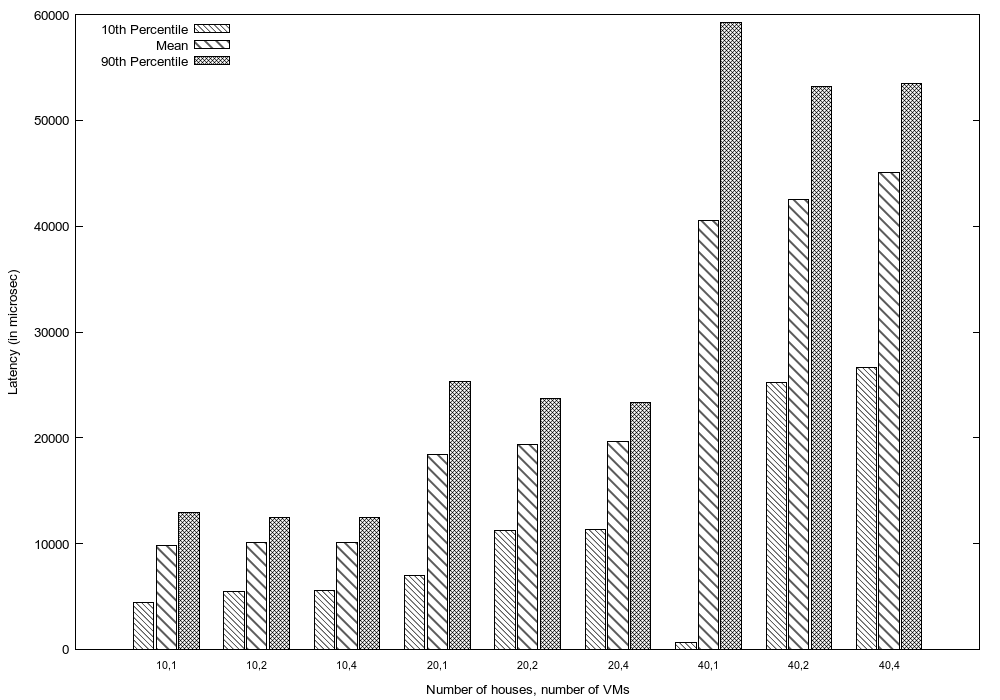
\includegraphics[scale=0.6]{img/q1_latency}
	\vspace*{-0.4cm}
	\caption{Latency vs No of Houses (Query 1) \label{fig:q1_latency}}
\end{center}
\end{figure}

\vspace*{-0.4cm}
As we increase the number of virtual machines, the latency values do not change much as shown in Figure \ref{fig:q1_latency}.
because the broker becomes the bottleneck.
The disk read in the broker limits the scalability of the system.
On the other hand, throughput remains nearly constant in all the experiments as shown in Figure \ref{fig:q1_throughput}.

\begin{figure}[h]
\begin{center}
	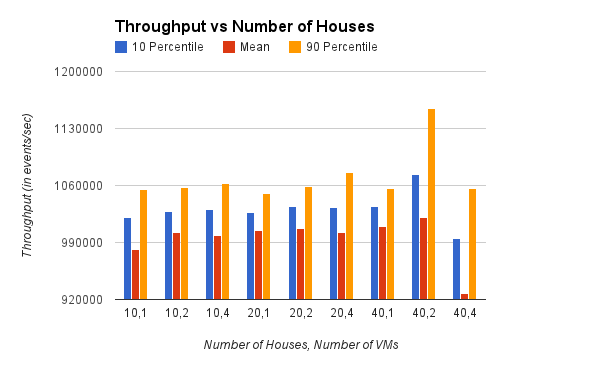
\includegraphics[scale=0.45]{img/q1_throughput}
	\vspace*{-0.4cm}
	\caption{Throughput vs No of Houses (Query 1)\label{fig:q1_throughput}}
\end{center}
\end{figure}

We contend based on utilization of CPU at the broker and house processes as evident from Figure \ref{fig:q1_util}, it is the broker that is currently limiting the scalability of the system.
The parsing of the read event accounts for most of the time spent by the broker on the CPU.
If we were getting events as a stream and can avoid both the disk I/O and conversion of strings to numbers, we can witness the scalability of the system as a whole since the house processes are separate and can be run on different cores.


\begin{figure}[h]
\begin{center}
	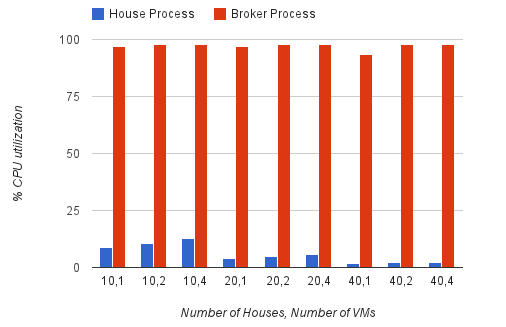
\includegraphics[scale=0.5]{img/q1_utilization}
	\vspace*{-0.4cm}
	\caption{\% Utilization vs No of Houses (Query 1)\label{fig:q1_util}}
\end{center}
\end{figure}
